
\chapter{Related Works}
\label{chapter:lit}
This chapter discusses various speech enhancement methods available in the literature. The different class of dereverberation methods available in the literature is summarized in Section~\ref{sec:dereverb_methods}. Since this work is based on NMF based model for reverberation and noise, the NMF based enhancement methods in the literature are explained in Section~\ref{sec:NMF_methods}.
%In this chapter we discusses various dereverberation methods available in literature. The different class of dereverberation methods available in literature is summarized in Section~\ref{sec:dereverb_methods}. Since this work is based on NMF based model for  reverberation and noise, the NMF based enhancement methods in literature are explained in Section~\ref{sec:NMF_methods}.

\section{Dereverberation methods}
\label{sec:dereverb_methods}


This section discusses various dereverberation methods in literature. Many of these methods can be extended to hande reverberation in presence of noise. The dereverberation methods can be broadly classified into - (i) beamforming, (ii) inverse filtering based methods, and (iii) reverberation suppression methods. Each methods are discussed in details next.

\subsection{Beamforming}

Beamforming is a multi-channel method. It utilizes the spatial information of the source and microphone array to enhance degraded speech recordings. A beamformer enhances the signal received from a particular direction and attenuates the signal received from other directions~\cite{naylor2010speech}. This spatial filtering is made possible by the fact that the sound waves travel an additional distance to reach distant microphones when compared with nearer microphones. This result in a relative time lag is referred to as time delay of arrival (TDAO). TDOA depends on the source position and microphone array configuration. 

Figure~\ref{fig:TDOA} illustrates the occurrence of TDOA for a source paced distant from a two-microphone array. 
The source is placed at an angle $\theta$ from the axis of the microphone array (referred to as incident angle). The signal travels an extra distance of $d\text{cos}(\theta)$ to reach microphone $M_1$ when compared with the reference microphone $M_{ref}$. This results in a time lag $\tau$ of
\begin{equation}
\tau = \dfrac{d \text{cos}(\theta)}{v}\text{,}
\end{equation}
where $v$ is velocity of sound in the medium. It can be observed that TDOA changed with the incident angle $\theta$ and microphone spacing $d$. 
\begin{figure}
\centering
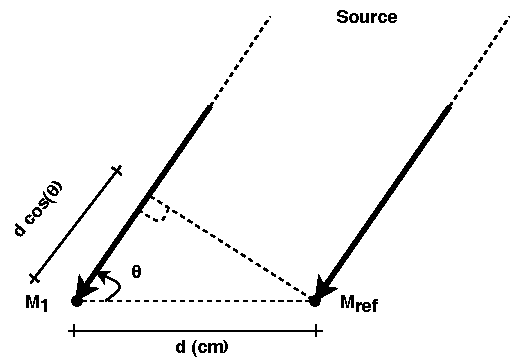
\includegraphics[width=\linewidth]{TDOA_plot.pdf}
\caption{ Two-microphone DSR recording setup. Microphones are placed $d$-distant apart. The effects of reverberation and noise is not shown in the figure.}
\label{fig:TDOA}
\end{figure}

Delay-sum beamforming (DSB) is the most straight forward beamforming approach. The microphone recordings are delayed to compensate for different TDOAs and a convex combination of these signals is taken. For a $M$-microphone array, the enhanced signal $\hat{x}(n)$ obtained using DSB can be summarized as,
\begin{equation}
\hat{x}(n)=\sum_{m=1}^M p_m x_m(n-\tau_m) \text{,}
\end{equation}
where $x_m(n)$ is the recording for $m$-th microphone. $p_m$ and $\tau_m$ represents the weight and TDOAs obtained for each microphone. $p_m$ can be fixed based on some amplitude normalization criteria~\cite{anguera2007acoustic}. $\tau_m$ can be estimated based on the source localization algorithms like generalized cross-correlation with phase transform (GCC-PHAT)~\cite{knapp1976generalized}. The signals from look-direction in different channels will add constructively. This results in enhancing signals coming from look-direction at the expense of the signals received from other directions.  Beamforming was shown to effectively suppress localized noise. However, reverberant speech is partially suppressed. Reverberation makes localized speech sources into diffused sound. The resulting reverberated speech signal reaches the array from all directions. Hence, reverberated speech signal coming from look direction will not be suppressed, while from other directions will be suppressed. 
 
Many modifications were proposed to improve the performance of the beamformer. MVDR beamforming uses noise statistics to improve performance. The effects of reverberation were suppressed with the use of multiple beamformers. This is achieved with the use of a three-dimensional microphone array. One beam is steered in the direction of the desired location as was the case in earlier.  Additional beams are steered in the direction of the strong initial reflections~\cite{nishiura2001speech} which acts as virtual sources. Another method to suppress reverberation was the use of a matched filter beamformer where the microphone responses are convolved with time-reversed RIR. The method requires Reverberation suppression methods model the effect of reverberation on the clean speech in some domains like the short-time Fourier transform (STFT), the residual signal obtained from linear prediction analysis, etc. Based on these models, algorithms are proposed to reduce the effects of reverberation. This results in a better estimate of clean speech. The approaches include spectral subtraction~\cite{lebart2001new}, weighted linear prediction (WPE)~\cite{nakatani2010speech}, Triple-N ICA for convolutive mixtures (TRINICON)~\cite{buchner2007trinicon}, linear prediction based method~\cite{naylor2010speech}, and NMF based approaches~\cite{kameoka2009robust}, information about RIR~\cite{naylor2010speech}.

\subsection{Inverse filtering based methods}
Inverse filtering based methods are multi-channel speech enhancement methods~\cite{naylor2010speech}. These methods have two steps - (i) blind estimation of RIR and (ii) inverse filtering.
\subsubsection{(i) Blind estimation of RIR}
\label{sec:MINT}
In this step, a blind estimate for RIR from the source to at least one of the microphones in the array is obtained. The correlation between speech recorded by different microphone channels is used for the purpose. Consider two channels DSR recording case degraded by reverberation alone. The microphone outputs $y_{R,1}$ and $y_{R,2}$ represented as,
\begin{align}
y_{R,1}(n)&=s(n)*h_1(n) \text{  and } \nonumber \\
y_{R,2}(n)&=s(n)*h_2(n)
\end{align}
where $s(n)$ is the clean speech, and $h_1(n)$ and $h_2(n)$ represents the RIRs form the source to the first and the second microphone, respectively. The microphone outputs are correlated based on the following relation.
\begin{align}
y_{R,1}(n)*h_2(n)&=(s(n)*h_1(n))*h_2(n) \nonumber \\
                 &=h_1(n)*(s(n)*h_2(n)) \nonumber \\
                 &=y_{R,2}(n)*h_1(n) \nonumber\\
y_{R,1}(n)*h_2(n)&-y_{R,2}(n)*h_1(n)=0
\label{eq:rir_cancel}
\end{align}
Based on (\ref{eq:rir_cancel}), a system of equations of the following form can be written~ \cite{xu1995least}.
\begin{equation}
\mathbf{Rh}=\mathbf{0}
\label{eq:system_eq}
\end{equation}
where, $\mathbf{R}$ represents a correlation-like matrix obtained from source signal $s(n)$~\cite{huang2003class}. $\mathbf{0}$ represents a zero vector. The vector $\mathbf{h}$ is obtained from RIRs as $\mathbf{h}=[\mathbf{h}_1^T|\mathbf{h}_2^T]^T$, where $h_1(n)$ and $h_2(n)$ form the elements of $\mathbf{h}_1$ and $\mathbf{h}_2$, respectively. The ideal solution for the $\mathbf{h}$ in the system of equations (\ref{eq:system_eq}) is the eigen-vector corresponding to the zeroth eigen-value in $\mathbf{R}$. In the presence of noise, the solution for $\mathbf{h}$ is eigen-vector corresponding to the smallest eigen-value. The system of equations in (\ref{eq:system_eq}) can be generalized for more microphone recordings are available.

Different approaches have been proposed in the literature to blindly estimate RIR based on the system of equations in (\ref{eq:system_eq}). Such methods assume that certain identifiability conditions and practical considerations are met~\cite{naylor2010speech}. Some of these methods are explained here. In~\cite{huang2003class}, a least-squares (LS) approach was proposed to solve the system of equations in (\ref{eq:system_eq}). The method based on eigendecomposition was also been proposed~\cite{gurelli1995evam}. In~\cite{gannot2003subspace}, full bands and frequency sub-bands eigendecomposition methods were proposed to solve for (\ref{eq:system_eq}) in the presence of white and colored noises. Adaptive filter in time domain~\cite{huang2002adaptive}  and frequency domain~\cite{huang2003class} were also proposed in literature.

\subsubsection{(ii) Inverse filtering}
\label{sec:inverse_fitering}
Inverse filtering methods could be used to estimate clean speech $s(n)$ from reverberated microphone recordings $y_{R,m}(n)$ and an estimate of RIRs $h_m(n)$. The most straight forward method would be to use an inverse filter $\mathbf{G}_m$ that  compensate for effects of reverberation as shown next.
\begin{equation}
\mathbf{y}_m^T\mathbf{G}_m=\alpha_0 \delta(n-n_0)\text{,}
\label{eq:direct_inversion}
\end{equation}
where $\alpha_0$ and $n_0$ represent arbitrary scaling and delay factors, respectively. $\delta(n)$ represents unit discrete delta function. However, the use of the direct inverse system shown in (\ref{eq:direct_inversion}) is challenging because of the following factors.  (i) RIR has non-minimum phase characteristics~\cite{neely1979invertibility}, (ii) spectral nulls can be present RIR spectrum and (iii) estimated inverse filter will have thousands of coefficients that require high precision and computationally expensive methods. In~\cite{mourjopoulos1982comparative}, inverse filter estimate $\hat{\mathbf{G}}_m$ was obtained based on a LS method. The estimated inverse filter minimizes the following cost function.
\begin{equation}
\hat{\mathbf{G}}_m = \underset{\mathbf{G}_m}{\text{min}} \left\lVert \mathbf{h}_m^T\mathbf{G}_m - \delta(n-n_0) \right\rVert_2^2
\end{equation} 
Homomorphic inverse filtering methods were also been investigated~\cite{radlovic2000nonminimum,mourjopoulos1982comparative}. The inverse filter was decomposed into minimum-phase and all-pass components. The minimum-phase component can be directly estimated from the magnitude spectrum of estimated RIR. Various methods like matched filtering~\cite{radlovic2000nonminimum} were used to estimate the all-pass components. 

When multi-channel RIRs are available, multiple-input/output inverse theorem (MINT) based approaches can be used to find exact inverse filters~\cite{miyoshi1988inverse}. According to the theorem, if the transfer function of two RIRs does not have any common zeros, then there exist a pair of inverse filters $\mathbf{G}_1$ and $\mathbf{G}_2$  such that
\begin{equation}
\mathbf{h}_1^T\mathbf{G}_1+\mathbf{h}_2^T\mathbf{G}_2=\delta(n)
\label{eq:MINT}
\end{equation}
In~\cite{miyoshi1988inverse}, a LS method was used to solve for (\ref{eq:MINT}). An exact inverse filtering can be performed by using an inverse filter length similar to that of RIR length. A sub-band version was proposed in~\cite{yamada1991recovering}. An adaptive version of the method is proposed in~\cite{nelson1995inverse}. Regularization was imposed on equalization problem in (\ref{eq:MINT}) to improve the robustness against noise and estimation errors~\cite{naylor2010speech}. 

\subsection{Reverberation suppression methods}
Reverberation suppression methods are based on modeling the effect of reverberation on clean speech in some domains. The commonly used domains are the short-time Fourier transform (STFT) and its variants, the residual signal obtained from linear prediction analysis, etc. Based on these degradation models, algorithms were proposed to reduce the effects of reverberation. This results in a better estimate of clean speech. The approaches include spectral subtraction~\cite{lebart2001new}, weighted linear prediction (WPE)~\cite{nakatani2010speech}, Triple-N ICA for convolutive mixtures (TRINICON)~\cite{buchner2007trinicon}, linear prediction based method~\cite{naylor2010speech}, and NMF based approaches~\cite{kameoka2009robust}, etc. SuchTypically these algorithms are single-channel methods. However, these methods can easily be extended for a multi-channel scenario.

\section{NMF based dereverberation methods}
\label{sec:NMF_methods}

NMF based speech enhancement methods are based on the modulation transfer function (MTF) model for reverberation. The MTF model states that for each frequency sub-band, the power envelope of the reverberated speech $\mathbb{Y}_R(k,n)$ is the convolution of power envelopes of clean speech $\mathbb{S}(k,n)$ and RIR $\mathbb{H}(k,n)$ for that particular sub-band. Mathematically,
\begin{equation}
\mathbb{Y}_R(k,n)=\mathbb{H}(k,n)*_n\mathbb{S}(k,n)=\sum_{l=0}^{L_h-1}\mathbb{H}(k,l)\mathbb{S}(k,n-l)\text{,}
\label{eq:MTF_model}
\end{equation}
where $*_n$ represents convolution along the time axis. $L_h$ represents the number of frames used to represent the RIR spectrogram. This model is valid when the reverberation condition does not change with time. Further, the MTF model is obtained by ignoring the cross-band effects occurring due to windowing~\cite{avargel2007system}.  The RIR phase spectrogram is also assumed to be uniformly distributed in the range $[-\pi, \pi)$.
Even though these approximations in the MTF model can pose a limitation for the dereverberation task, many dereverberation methods use this model. An additional advantage of the MTF model is that it avoids the need for a phase estimate for the RIR. Obtaining the phase spectrogram is difficult, especially if the recording is noisy~\cite{kameoka2009robust}. Estimation of $\mathbb{H}(k,n)$ and $\mathbb{S}(k,n)$ from $\mathbb{Y}_R(k,n)$ in (\ref{eq:MTF_model}) is viewed as solving for a CNMF problem. The dereverberated speech obtained using this algorithm showed improvements in speech enhancement instrumental measures.

Many modifications were proposed to improve the performance. The use of a magnitude spectrogram instead of a power spectrogram showed superior performance~\cite{Kumar2011}. The magnitude spectrogram of reverberated speech $\mathbf{Y}_R$ is expressed as a convolution of magnitude spectrograms of clean speech $\mathbf{S}$ and RIR $\mathbf{H}$. Mathematically,
\begin{align}
\mathbf{Y}_R&=\mathbf{H}*_n\mathbf{S} \nonumber \\
Y_R(k,n)& = \sum_{l=0}^{L_h-1} H(k,l)S(k,n-l) \text{,}
\label{eq:cnmf0}
\end{align}
where, $Y_R(k,n)$ $H(k,n)$, and $S(k,n)$ represents the elements of $\mathbf{Y}_R$, $\mathbf{H}$ and $\mathbf{S}$, respectively. Further, it was shown that the use of gamma-tone filter banks helped in improving ASR results when compared with the use of uniform filter banks. 

The reverberation model in (\ref{eq:cnmf0}) did not use any model for the clean speech spectrogram. Introducing clean speech spectrogram models were shown to improve speech enhancement results.  In~\cite{mohammadiha2016speech, Mohammadiha2015}, a NMF model for the clean speech spectrogram $\mathbf{S}$ was incorporated in the reverberation model in (\ref{eq:cnmf0}). The NMF model of clean speech spectrogram can be written as,
\begin{align}
\mathbf{S}&= \mathbf{W}_s\mathbf{X}_s \nonumber \\
S(k,n)    &= \sum_{r=1}^{R_s} W_s(k,r)X_s(r,n)\text{,}
\label{eq:NMF_clean_speech}
\end{align}
where, $\mathbf{W}_s$ and $\mathbf{X}_s$ represents bases and activation matrices obtained by performing NMF decomposition on the clean speech spectrogram $
\mathbf{S}$, respectively. $R_s$ represents the rank of NMF decomposition. $W_s(k,r)$ and $X_s(r,n)$ represents the elements of $\mathbf{W}_s$ and $\mathbf{X}_s$, respectively. Incorporating the clean speech model (\ref{eq:NMF_clean_speech}) in the reverberation model in (\ref{eq:cnmf0}) results in a reverberation model that can be written as,
\begin{equation}
Y_R(k,n) = \sum_{l=0}^{L_h-1} H(k,l) \bigg[ \sum_{r=1}^{R_s} W_s(k,r) X_s(r,n-l) \bigg]
\label{eq:cnmf1}
\end{equation}
Iterative algorithm were proposed to estimate clean speech spectrogram. There were two approaches depending on how clean speech bases $\mathbf{W}_s$ is learned - online approach and offline approach. In offline approach , the $\mathbf{W}_s$ is learned from reverberated spectrogram. In online approach, $\mathbf{W}_s$ is pre-learned from a set of clean speech utterances. A NMF decomposition is performed on the magnitude spectrogram of these clean speech utterances to estimate $\mathbf{W}_s$. Many constraints on the estimated clean speech like sparsity~\cite{mohammadiha2016speech, Mohammadiha2015}, and continuity~\cite{wager2018collaborative} were used to improve the performance. 

Representing clean speech spectrogram using CNMF model were also proposed to improve speech dereverberation perfromance~\cite{Mirsamadi2014}. In~\cite{Kallasjoki2014}, a NMF model for speech reverberation was proposed. This model is equivalent to the CNMF model for reverberation in (\ref{eq:cnmf1}). The bases matrix of the NMF decomposition is a structured matrix that was constructed to mimics the CNMF model.

The reverberation model in (\ref{eq:cnmf1}) is inappropriate to model reverberation in the presence of noise.  The model was modified by incorporating a noise model. The magnitude spectrogram of reverberated speech in the presence of noise $\mathbf{Y}$ was approximated as the sum of magnitude spectrograms of reverberated speech $\mathbf{Y}_R$ and noise $\mathbf{Z}$~\cite{li2018multichannel}. Mathematically,
\begin{align}
\mathbf{Y} &\approx \mathbf{Y}_R+\mathbf{Z} = \mathbf{H}*_n\mathbf{S}+\mathbf{Z}\nonumber \\
Y(k,n) &= H(k,n)*_n S(k,n) + Z(k,n) \text{,}
\label{eq:degradation_model}
\end{align}
where $Y(k,n)$ and $Z(k,n)$ represents the elements of $\mathbf{Y}$ and $\mathbf{Z}$, respectively. Similar to the NMF model for clean speech spectrogram in (\ref{eq:NMF_clean_speech}), a NMF approximation for noise spectrogram can be used as shown in (\ref{eq:NMF_noise}).
\begin{align}
\mathbf{Z}&= \mathbf{W}_n\mathbf{X}_n \nonumber \\
Z(k,n)    &= \sum_{r=1}^{R_n} W_n(k,r)X_n(r,n)\text{,}
\label{eq:NMF_noise}
\end{align}
where $\mathbf{W}_n$ and $\mathbf{X}_n$ were the bases and activation matrix of noise spectrogram $\mathbf{Z}$. $R_n$ represents the rank of NMF decomposition. $W_n(k,r)$ and $X_n(r,n)$ represents the elements of $\mathbf{W}_n$ and $\mathbf{X}_n$, respectively. The  degradation model in (\ref{eq:degradation_model}) is modified with the use of NMF models for clean speech in (\ref{eq:NMF_clean_speech}) and noise (\ref{eq:NMF_noise}) as shown next.
\begin{align}
\mathbf{Y} & = \mathbf{H}*_n \bigg[ \mathbf{W}_s\mathbf{X}_s \bigg]+\mathbf{W}_n\mathbf{X}_n
\label{eq:NMF_degradation_model}
\end{align}
Based on the degradation model in (\ref{eq:NMF_degradation_model}), a speech enhancement algorithm was proposed in~\cite{baby2016supervised}. The algorithm was a supervised approach where the clean speech and noise bases are assumed to be known. Exemplar-bases are learned for the purpose. This approach of obtaining the bases is different from the one used in~\cite{mohammadiha2016speech, Mohammadiha2015}. The use of the CNMF model for the clean speech and the noise spectrogram was also proposed in~\cite{baby2016supervised, baby2016phd}. The use of the CNMF model for the clean speech and the noise spectrogram was also proposed in~\cite{baby2016supervised, baby2016phd}. In~\cite{baby2016supervised}, the temporal variation of the RIR spectrogram was modeled along with the degradation model in (\ref{eq:NMF_degradation_model}).

\iffalse
\begin{itemize}
\item Reverberation methods: cost function, iterative procedure
\item Extending to noisy scenario - use of additive noise, extended model, results
\end{itemize}
\fi

\section{Limitations of NMF based dereverberation methods in literature}
The NMF based speech enhancement methods in literature utilize limited information about the RIR spectrogram.  This limits the performance of these algorithms. In this work different spectro-temporal models for the RIR spectrograms are proposed. Incorporating these novel RIR constraints on the NMF based enhancement algorithm helped in improving the performance. The reverberation models used in this work models the effects of reverberation on the magnitude spectrogram of clean speech. Hence, in the subsequent chapters, the usage of spectrogram means the magnitude spectrogram, unless stated otherwise. 
Chapter~\ref{chapter:rir} discusses the various properties of the RIR. Some of these properties are used in this work. The subsequent chapters discuss the different proposed speech enhancement algorithms that utilize these RIR models.  

\iffalse
\begin{itemize}
\item Most methods does not model RIR
\item Some methods use week constraints on RIR 
\item Thesis work is on incorporation various models for RIR in NMF based reverberation model
\item This resulted in improved enhancement and ASR results, proper RIR estimates 
\end{itemize}
\fi

\iffalse
Speech originating from a source undergoes multiple reflections in a closed room. When this speech is captured using a microphone distant from the source (typically 30 cm to few meters), the microphone output is a superposition of the speech along with the delayed and attenuated copies of the signal referred to as reverberated speech~\cite{naylor2010speech}. Additionally, the microphone will capture background noise originating from other sources. The resulting microphone output in such a distant speech recording (DSR) setting is a degraded version of the original speech signal. The presence of such degradations impedes speech intelligibility~\cite{kinoshita2016summary}  and automatic speech recognition (ASR)~\cite{barker2018fifth, barker2015third} performance. The amount of degradation depends on the source and microphone positions, characteristics of the room and the noise~\cite{naylor2010speech,kinoshita2016summary}. To improve performance, it is desirable to compensate for these degradations. The focus of this work is on jointly handling dereverberation and denoising. In this work we refer to methods that perform dereverberation in presence of noise as speech enhancement methods.

Dereverberation methods in literature can be broadly classified as (i) beamforming methods, (ii) inverse filtering methods and (iii) reverberation suppression methods. Many of these approaches can be extended to jointly handle reverberation and noise. (i) Beamforming is a multi-channel method. It uses a spatial filter that enhances speech incident from the desired direction and suppresses speech coming from other directions~\cite{gannot2017consolidated}. The multi-channel recordings are filtered and weighed to focus the beam to the desired direction. (ii) Inverse filtering methods blindly estimate the room impulse response (RIR) from the microphone recordings. Blind system identification approaches like the least-squares (LS) method and eigendecomposition method are used to blindly estimate the RIR~\cite{naylor2010speech}. This RIR is used to retrieve the original speech source. (iii) Reverberation suppression methods model the effect of reverberation on the clean speech in some domains like the short-time Fourier transform (STFT), the residual signal obtained from linear prediction analysis, etc. Based on these models, algorithms are proposed to reduce the effects of reverberation. This results in a better estimate of clean speech. The approaches include spectral subtraction~\cite{lebart2001new}, weighted linear prediction (WPE)~\cite{nakatani2010speech}, Triple-N ICA for convolutive mixtures (TRINICON)~\cite{buchner2007trinicon}, linear prediction based method~\cite{naylor2010speech}, and NMF based approaches~\cite{kameoka2009robust}, etc. In this work, a novel single-channel NMF based method to perform dereverberation and denoising jointly is proposed. Various NMF based enhancement methods proposed in literature are discussed next. 

NMF based dereverberation methods are based on the non-negative convolutive transfer function (N-CTF) model for the magnitude STFT of the reverberated speech ~\cite{kameoka2009robust,mohammadiha2016speech, Mohammadiha2015, Kumar2011}. For each frequency band, the temporal variation of reverberated speech is modeled as the convolution of magnitude spectrogram values of the clean speech and the RIR for that particular frequency. This model is valid when the reverberation condition does not change with time. Further, the N-CTF model is obtained by ignoring the cross-band effects occurring due to windowing~\cite{avargel2007system}.  Even though these approximations in the N-CTF model can pose a limitation for the dereverberation task, many dereverberation methods use this model. An additional advantage of the N-CTF model is that it avoids the need for a phase estimate for the RIR. Obtaining the phase spectrogram is difficult, especially if the recording is noisy~\cite{kameoka2009robust}. 

Based on the N-CTF model, a speech dereverberation algorithm was proposed in~\cite{kameoka2009robust}. Estimation of clean speech spectrogram is viewed as solving a CNMF problem. This algorithm shows improvements in speech enhancement instrumental measures. In~\cite{Kumar2011}, the N-CTF model for reverberation is extended for a gammatone filterbank. The estimated clean speech features are shown to improve ASR performance. In~\cite{Kallasjoki2014}, a NMF model for speech reverberation is proposed which is equivalent to the CNMF model for reverberation. The bases matrix of the NMF decomposition is a structured matrix that mimics the CNMF model. 
The dereverberation performance using the CNMF model was improved by introducing models for clean speech spectrograms like NMF~\cite{mohammadiha2016speech, Mohammadiha2015} and CNMF~\cite{Mirsamadi2014} models. Many constraints on the estimated clean speech are used like sparsity~\cite{mohammadiha2016speech, Mohammadiha2015}, and continuity~\cite{wager2018collaborative} to improve the performance.

The N-CTF model cannot be used as such for reverberated speech in the presence of noise. Including a noise model to the N-CTF model helps in improving the dereverberation performance. The magnitude spectrogram of reverberated speech in the presence of noise is approximated as the sum of magnitude spectrograms of reverberated speech and noise~\cite{li2018multichannel}. Using this model, with NMF models for clean speech and noise spectrograms, a supervised joint dereverberation and denoising algorithm was proposed in~\cite{baby2016supervised}. The use of the CNMF model for the clean speech and the noise spectrogram was also proposed in~\cite{baby2016supervised, baby2016phd}. All the enhancement methods based on N-CTF discussed above use models for clean speech spectrogram but do not use any specific models for the RIR spectrogram.

Use of meaningful constraints on the RIR spectrogram along with speech model will help the dereverberation methods. Some methods use a simple model for the RIR spectrogram. The temporal variation of the RIR spectrogram was modeled in~\cite{baby2016supervised}. The RIR spectrogram energy across frames was modeled to decay with time. Based on this RIR model, an enhancement algorithm was proposed in~\cite{baby2017joint}, to improve the speech enhancement results. This method does not consider the spectral variation of the RIR spectrogram. With the knowledge of the RIR, we had proposed in~\cite{mohanan2017speech}, the use of the sparse nature and the presence of a frequency envelope for the RIR spectrogram to improve the speech enhancement results. Further, in~\cite{mohanan201a}, a spectral and temporal model for the RIR spectrogram was proposed based on a separability approximation on the RIR spectrogram. The approximation resulted in a rank-$1$ NMF model for the RIR spectrogram. Based on the RIR model, the reverberated speech spectrogram is modeled using NMF as opposed to CNMF model used in literature.

In this work, we propose a NMF based approach to handle dereverberation and denoising jointly. Such an approach is different from other NMF based approaches that use a combination of CNMF and NMF for the purpose. The proposed model is easy to interpret. The spectral and temporal variation of the RIR is modeled using a low-rank NMF approximation of the RIR spectrogram. Even though such a representation reduces the number of parameters used for representing the RIR spectrogram, the enhancement results obtained are better than other NMF based approaches. Further, the approach is extended to work in unknown noise conditions. Such an approach gives better enhancement results when compared to existing NMF based dereverberation methods. As a byproduct, the RIR spectrogram estimates obtained using the proposed approach is better and closer to the true RIR spectrogram when compared to other NMF based approaches.

The main contribution of this paper is in incorporating a novel spectro-temporal model for the RIR spectrogram in the N-CTF model for reverberation. This model results in a NMF based algorithm to jointly handle dereverberation and denoising. Such a representation helps in imposing better constraints on the RIR spectrogram which was not possible in other NMF based methods. This resulted in superior enhancement results when compare with competing methods.
%The proposed algorithm showed superior enhancement results. 
This also resulted in a RIR estimate which is closer to the true RIR spectrogram.
\fi